% \strip{color}{sector angle}{sector number}{outer_radius}{inner_radius}
\tikzstyle{wired}=[draw=gray!30, line width=0.15mm]
\newcommand{\strip}[5]{
	\filldraw[#1,wired]
	({(#2) *  (#3)}		:						{(#5)}	) arc
	({(#2) *  (#3)}		:	{(#2) * ((#3) + 1)}	:	{(#5)}	) --
	({(#2) * ((#3) + 1)}	:						{(#4)}	) arc
	({(#2) * ((#3) + 1)}	:	{(#2) *  (#3)}		:	{(#4)}	) -- cycle;
}
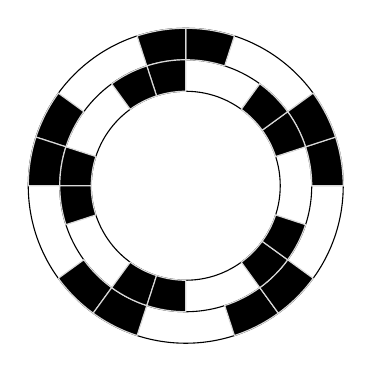
\begin{tikzpicture}
\pgfmathsetmacro{\scale}{2}
\pgfmathsetmacro{\parts}{5}
\pgfmathsetmacro{\posOut}{1}
\pgfmathsetmacro{\posMiddle}{0.8}
\pgfmathsetmacro{\posIns}{0.6}

\pgfmathsetmacro{\circles}{\parts*4}
\pgfmathsetmacro{\posOut}{1 * \scale}
\pgfmathsetmacro{\posMiddle}{0.8 * \scale}
\pgfmathsetmacro{\posInside}{0.6 * \scale}
\pgfmathsetmacro{\partAngle}{360 / \circles}
\path (0,0)[draw=black] circle (\posOut);
\path (0,0)[draw=black] circle (\posMiddle);
\path (0,0)[draw=black] circle (\posInside);
\foreach\i in {0,4,...,\circles} {
    \strip{black}{\partAngle}{\i + 0}{\posMiddle}{\posOut}
    \strip{black}{\partAngle}{\i + 1}{\posMiddle}{\posOut}
    \strip{black}{\partAngle}{\i + 1}{\posInside}{\posMiddle}
    \strip{black}{\partAngle}{\i + 2}{\posInside}{\posMiddle}
}
\end{tikzpicture}
